\documentclass[12pt]{report}
\usepackage[T1]{fontenc}
\usepackage[french]{babel}
\usepackage[utf8x]{inputenc}
\usepackage{amsmath}
\usepackage{graphicx}
\usepackage[colorinlistoftodos]{todonotes}
\usepackage[strings]{underscore}
\usepackage{url}
\usepackage{hyperref}
\hypersetup{%
    pdfborder = {0 0 0}
}

\begin{document}



%-----------------------------------------------------------------%
%    PAGE DE TITRE
%-----------------------------------------------------------------%

\begin{titlepage}

\newcommand{\HRule}{\rule{\linewidth}{0.7mm}} % Trait horizontal

\center
 
%---------------------------%
%   LOGO & EN-TÊTE DE PAGE
%---------------------------%

\includegraphics[width=0.8\textwidth]{img/logo.jpg}\\

\textsc{\Large Projet de Programmation}\\[0.5cm]
\textsc{\large Génération procédurale de planètes}\\[0.5cm]

%---------------------------%
%   TITRE
%---------------------------%

\HRule \\[0.4cm]
{ \huge \bfseries Rapport}\\[0.4cm]
\HRule \\[1.5cm]
 
%---------------------------%
%   AUTHEURS
%---------------------------%

\begin{minipage}{0.4\textwidth}
\begin{flushleft} \large
\emph{Auteurs:}\\
Rémy \textsc{Maugey}\\
Jérémi \textsc{Bernard}\\
Hugo \textsc{Alonso}\\
Brian \textsc{Mazé}\\
\end{flushleft}
\end{minipage}
~
\begin{minipage}{0.4\textwidth}
\begin{flushright} \large
\emph{Client:} \\
Emmanuel \textsc{Fleury}
\end{flushright}
~
\begin{flushright} \large
\emph{Chargé de TD:} \\
Boris \textsc{Mansencal}
\end{flushright}
\end{minipage}\\[2cm]

%---------------------------%
%   DATE
%---------------------------%

{\large 05 Avril 2018\\[2cm] }


\vfill % Fill the rest of the page with whitespace

\end{titlepage}
%-----------------------------------------------------------------%
%   FIN PAGE DE TITRE
%-----------------------------------------------------------------%









%-----------------------------------------------------------------%
%   Table des Matières
%-----------------------------------------------------------------%


\tableofcontents

\thispagestyle{empty} % empeche l'affichage du numero de cet page

















%-----------------------------------------------------------------%
%   Introduction
%-----------------------------------------------------------------%

\newpage

\chapter*{Introduction}
\addcontentsline{toc}{chapter}{Introduction}
\setcounter{chapter}{1}














%-----------------------------------------------------------------%
%   Algorithme CDLOD
%-----------------------------------------------------------------%


\newpage

\chapter*{Algorithme CDLOD}
\addcontentsline{toc}{chapter}{Algorithme CDLOD}

L'algortihme \textbf{CDLOD}, pour "Continuous Distance-Dependent Level of Detail for Rendering Heightmaps " ( 
Niveau de détail continu dépendant de la distance pour le rendue de carte de hauteur") par Filip Strugar, est un algorithme qui comme sont nom l'indique, se base sur la distance pour l'affichage du niveau de détail (\textbf{LOD}) basé sur une carte de hauteur (\textbf{Heightmaps}).

De nombreux algorithme se servent de niveau de détail pour générer leur terrain mais un des problèmes majeurs auxquels ils se confrontent viens dès lors de la séparation entre deux niveau de détail voisins. 
\begin{wrapfigure}[5]{r}{6cm}
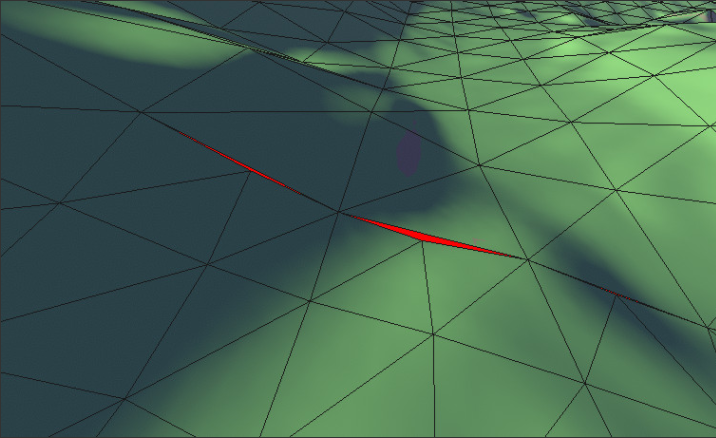
\includegraphics[width=6cm]{img/seams.png}
  \caption{Discontinuité}
  \label{fig:seams}
  \source {http://mikejsavage.co.uk/blog/geometry-clipmaps.html}
\end{wrapfigure}

\vspace{0.5cm}
En effet la différence d'élévation entre chaque divisions peuvent provoqué une discontinuité provoquant ainsi une zone vide, comme on peut le voir, par la zone rouge indiqué sur cette image. 


\vspace{3.2cm}
La méthode utilisé en général est de palier cette discontinuité en rajoutant des connexions entre les niveaux affectés. Cette solution à de nombreux inconvéniant, en rajoutant des connexions de cet manière, lors du rendue et du parcours du terrain ,ces connexions vont alors apparaitre brusquement perturbant ainsi la fluidité. À cela viennent s'ajouter la possibilité d'avoir des connexions multiple superposé et également un cout de rendue suplémentaire en terme de calcul et de mémoire.

Pour résoudre ce problème l'algorithme CDLOD va ici venir se servir de "transitions" entre les niveaux de détails par une méthode dites de "morphing"

\end{document}











































%-----------------------------------------------------------------%
%   END
%-----------------------------------------------------------------%

\end{document}